\documentclass{article}

\usepackage{arxiv}

\usepackage[utf8]{inputenc}
\usepackage[T1]{fontenc}
\usepackage{hyperref}
\usepackage{url}
\usepackage{booktabs}
\usepackage{amsfonts}
\usepackage{amsmath}
\usepackage{amssymb}
\usepackage{nicefrac}
\usepackage[babel=true]{microtype}
\usepackage{cleveref}
\usepackage{graphicx}
\usepackage{natbib}
\usepackage{doi}
\usepackage{multirow}
\usepackage{array}
\usepackage{algorithm}
\usepackage{algorithmic}

\title{PhyCL-Net: Physics-Inspired Contrastive Lightweight Network for Wearable Fall Detection}

\newif\ifuniqueAffiliation
\uniqueAffiliationtrue

\ifuniqueAffiliation
\author{
	Bowen Zuo\textsuperscript{1}, Siqi Wang\textsuperscript{1}, Junhui Xie\textsuperscript{1}, Sihan Liu\textsuperscript{1}, Xiaojuan Luo\textsuperscript{1,*}\\
	\textsuperscript{1}East China University of Science and Technology, Shanghai 200237, China\\
	\textsuperscript{*}Corresponding author: \texttt{luoxj@ecust.edu.cn}
}
\fi

\renewcommand{\shorttitle}{PhyCL-Net: Lightweight Fall Detection}

\hypersetup{
pdftitle={PhyCL-Net: Physics-Inspired Contrastive Lightweight Network for Wearable Fall Detection},
pdfsubject={cs.LG, cs.CV},
pdfauthor={Bowen Zuo, Siqi Wang, Junhui Xie, Sihan Liu, Xiaojuan Luo},
pdfkeywords={fall detection, wearable sensors, lightweight deep learning, dynamic kernels, attention, contrastive learning, edge inference},
}

\begin{document}
\maketitle

\begin{abstract}Deploying high-performance fall detection on resource-constrained wearable devices faces an accuracy-efficiency dilemma: while time-frequency analysis (e.g., MSPA) yields high performance, it incurs prohibitive computational costs for edge deployment. We propose \textbf{PhyCL-Net}, a purely time-domain lightweight network that eliminates the heavy spectral processing branch. Instead, it relies on (i) \textit{Physics-Guided Dynamic Kernel selection (PDK)} to adapt temporal receptive fields to the impulse response characteristics of falls, and (ii) \textit{Fall-Aware Attention (FAA)} to emphasize transient impact cues (Jerk) while suppressing sustained high-intensity activities. A cross-gated fusion module integrates these branches with minimal overhead. During training, we employ a hierarchical dual-view contrastive objective and center regularization to enhance class separability, which are removed at inference to maintain zero deployment cost. Evaluated on the SisFall dataset (12-subject subset, young adults aged 19--30) using a strict leave-one-subject-out (LOSO) protocol, PhyCL-Net achieves \textbf{98.20\% accuracy} and \textbf{98.15\% macro-F1}. Crucially, compared to the frequency-heavy AMSNetV2\footnote{AMSNetV2 is our prior work that combines multi-scale spectral pyramid analysis (MSPA) with adaptive temporal modeling. The key difference from PhyCL-Net is the explicit frequency-domain processing branch.} backbone, PhyCL-Net reduces parameter count from 1.66M to \textbf{1.04M} ($-37.0\%$) and cuts CPU inference latency from 184.31\,ms to \textbf{125.99\,ms} ($-31.6\%$), offering a superior trade-off for TinyML applications. \textbf{Limitations:} This work evaluates PhyCL-Net on laboratory data from young adults (ages 19--30, $n=12$) using a single waist-mounted tri-axial accelerometer. Critical limitations include: (1) lack of validation in elderly populations with age-related fall biomechanics, (2) absence of real-world uncontrolled environment testing, and (3) no quantification of impact on other sensor placements. Clinical deployment requires further validation with target users. \textbf{Code:} \url{https://github.com/AlexZander-666/phycl-net-fall-detection}\end{abstract}

\keywords{fall detection \and wearable sensors \and lightweight deep learning \and contrastive learning \and edge inference}

\section{Introduction}

Falls are a leading cause of injury-related morbidity and mortality among older adults worldwide, creating an urgent need for automated detection systems~\cite{world2021falls,Newaz2023Methods}. Wearable inertial sensors (accelerometers and gyroscopes) have emerged as the most practical safety layer for continuous monitoring due to their low cost, privacy-preserving nature, and ubiquity in smart devices~\cite{Igual2013Challenges,Chaccour2017Sensors,Casilari2015Wearable}. With the rapid expansion of the Internet of Health Things (IoHT), the paradigm is shifting from cloud-centric processing to \textit{Edge AI}—processing data directly on the wearable node to ensure low latency and offline reliability~\cite{Ramachandran2020Survey,Guo2016Practical}.

However, deploying robust deep learning models on battery-powered edge devices presents a severe \textbf{Accuracy--Efficiency Dilemma}. Recent State-of-the-Art (SOTA) approaches primarily focus on increasing model capacity, utilizing heavy Transformers~\cite{Wang2024Survey,Zerveas2021TST,Wen2023PatchTST}, complex ensemble methods~\cite{Hussain2023Enhanced}, or explicit time--frequency representations (e.g., Spectrograms, Wavelets)~\cite{wang2019deep,mubashir2013survey}. While these methods achieve high accuracy, they often incur high computational costs (FLOPs) and memory footprints that exceed the constraints of typical Cortex-M microcontrollers used in wearables~\cite{Banbury2021TinyML}.

This work challenges the prevailing assumption that complex frequency-domain analysis is necessary for fall detection. Recent works like ModernTCN~\cite{luo2024moderntcn} have demonstrated that modernized convolutional structures can outperform Transformers in time-series tasks while remaining computationally efficient. From a \textbf{physical kinematics} perspective, routine Activities of Daily Living (ADLs) like walking or jogging are characterized by quasi-periodic low-frequency signals. In contrast, a fall's defining characteristic is the rapid change in acceleration (Jerk magnitude exceeding threshold), which manifests as a high-frequency transient during the 200--800\,ms impact phase~\cite{Bourke2007Threshold,Kangas2008Comparison}. To distinguish falls from high-intensity ADLs (e.g., jumping), we leverage Jerk as the discriminative cue. Transforming such a short, singular transient into the frequency domain (via STFT or spectral pyramids) can diffuse sharp temporal features and introduce unnecessary computational overhead. We hypothesize that a streamlined time-domain encoder, if designed to dynamically adapt to these impulse transients, can achieve SOTA accuracy without the burden of spectral processing.

Guided by this hypothesis, we propose \textbf{PhyCL-Net} (Physics-Inspired Contrastive Lightweight Network). Unlike its predecessor AMSNetV2 (our prior work combining multi-scale spectral pyramid analysis with adaptive temporal modeling), PhyCL-Net strategically removes the computationally expensive Multi-Scale Spectral Pyramid (MSPA). Instead, it relies on two lightweight, physics-aware mechanisms:

\begin{enumerate}
\item \textbf{Physics-Guided Dynamic Kernel (PDK) Selection:} A module that mimics the eye's accommodation reflex. It dynamically routes information through small kernels (to capture high-frequency impact transients) or large kernels (to capture low-frequency posture transitions) based on the signal's complexity.
\item \textbf{Fall-Aware Attention (FAA):} A mechanism explicitly designed to highlight "Jerk" (rapid derivative changes) and suppress high-energy but sustained ADLs (e.g., running).
\end{enumerate}

To compensate for the reduced parameter count, we introduce a \textbf{training-only} Hierarchical Dual-View Contrastive Learning (HDVCL) framework, building upon recent advances in time-series contrastive learning~\cite{Eldele2021TSTCC,Zhang2022TFC,Zheng2023SimTS}. This "Free Lunch" strategy forces the model to learn more discriminative embeddings during training, allowing us to strip away the auxiliary projection heads during inference, ensuring zero extra deployment cost.

\textbf{Contributions:}
\begin{itemize}
\item \textbf{Pure Time-Domain Efficiency:} We demonstrate that removing the spectral branch (MSPA) and relying on physics-guided temporal processing reduces parameters by \textbf{36.7\%} (1.05M vs. 1.66M) and CPU latency by \textbf{31.6\%} (126ms vs. 184ms) while maintaining statistical parity in accuracy.
\item \textbf{Physics-Inspired Architecture:} We propose the PDK and FAA modules, which functionally substitute spectral analysis by explicitly modeling the impulse and derivative characteristics of falls in the time domain.
\item \textbf{Deployment-Oriented Optimization:} We utilize a contrastive regularization strategy that improves safety-critical metrics (TPR@FPR=1\%) without adding inference parameters.
\item \textbf{Rigorous Validation:} On the SisFall dataset (12-subject subset), PhyCL-Net achieves \textbf{98.20\%} accuracy and \textbf{98.15\%} Macro-F1 under a strict Leave-One-Subject-Out (LOSO) protocol, validated with bootstrap confidence intervals.
\end{itemize}


\section{Methodology}

\subsection{Problem Formulation}

Let $\mathcal{D} = \{(\mathbf{X}_i, y_i)\}_{i=1}^N$ be the dataset, where $\mathbf{X}_i \in \mathbb{R}^{C \times L}$ represents a sliding window of inertial sensor data with $C$ channels (e.g., $C=3$ for tri-axial accelerometer) and length $L$. The label $y_i \in \{0, 1\}$ denotes ADL or Fall. Our goal is to learn a lightweight mapping $f_\theta: \mathbb{R}^{C \times L} \to [0,1]$ that maximizes sensitivity to impact transients while minimizing computational operations (FLOPs) and parameters $\theta$.

\subsection{PhyCL-Net Architecture Overview}

To resolve the accuracy--efficiency dilemma, PhyCL-Net abandons the traditional computationally expensive spectral transformation (MSPA). Instead, it adopts a dual-branch time-domain topology:
\begin{itemize}
\item \textbf{Branch A: Physics-Guided Dynamic Kernel (PDK):} Adapts the temporal receptive field size to match the signal's rate of change (Impulse vs. Stationary).
\item \textbf{Branch B: Fall-Aware Attention (FAA):} Focuses on high-order kinematic features (Jerk/Snap) to distinguish falls from high-intensity ADLs.
\end{itemize}
These branches are fused via a lightweight Cross-Gated mechanism. The network follows a hierarchical structure with three stages, progressively downsampling temporal resolution while increasing channel capacity ($64 \to 128 \to 256$).

\subsection{Physics-Guided Dynamic Kernel (PDK) Selection}

Falls are multi-scale physical events: they contain high-frequency impact spikes (requiring small temporal receptive fields) and low-frequency pre-fall/post-fall posture changes (requiring large receptive fields). Fixed-size convolutions (e.g., standard ResNet) fail to capture both simultaneously without stacking many layers.

Inspired by Selective Kernel Networks (SKNet)~\cite{li2019sknet}, conditionally parameterized convolutions~\cite{Yang2019CondConv}, and the visual accommodation reflex, we propose the PDK module. It dynamically routes input $\mathbf{X}$ through a bank of parallel 1D depthwise kernels $\mathcal{K} = \{k_1, k_2, \dots, k_M\}$ with varying sizes (e.g., $k \in \{7, 15, 31, 63\}$).

Let $\tilde{\mathbf{U}}_m = \text{DWConv}_{k_m}(\mathbf{X})$ be the output of the $m$-th kernel. We compute a global context descriptor $\mathbf{s} \in \mathbb{R}^C$ via Global Average Pooling (GAP). A lightweight router generates channel-wise attention weights $\mathbf{a} \in \mathbb{R}^{C \times M}$:
\begin{equation}
\mathbf{a} = \text{Softmax}(\mathbf{W}_2 \cdot \delta(\mathbf{W}_1 \cdot \mathbf{s}))
\end{equation}
where $\mathbf{W}_1, \mathbf{W}_2$ are dimensionality-reduction layers and $\delta$ is ReLU. The final output $\mathbf{Y}_{\text{PDK}}$ is the adaptively aggregated signal:
\begin{equation}
\mathbf{Y}_{\text{PDK}} = \sum_{m=1}^M \mathbf{a}_m \odot \tilde{\mathbf{U}}_m
\end{equation}

By assigning higher weights to small kernels ($k=7$) during impacts and large kernels ($k=63$) during ADLs, PDK functionally substitutes the multi-scale frequency analysis of MSPA with significantly lower latency.

\subsection{Fall-Aware Attention (FAA)}

While PDK handles temporal scale, distinguishing a ``Fall'' from a ``Jump'' requires kinematic context. Physically, falls are characterized by sudden changes in acceleration (Jerk, the first derivative of acceleration), which manifests as a high-frequency transient during the 200--800\,ms impact phase. Standard attention mechanisms often focus on raw magnitude, which can be confusingly similar between a jump and a fall. We explicitly extend attention mechanisms to kinematic derivatives (Jerk) for fall detection, enabling the model to distinguish impact transients from sustained high-intensity activities.

Building on attention mechanisms for efficient networks~\cite{woo2018cbam,hou2021coordinate}, the FAA module explicitly computes a "Jerk-Aware" attention map. We first approximate the temporal derivative of the feature map $\mathbf{F}$:
\begin{equation}
\Delta \mathbf{F}_t = \mathbf{F}_t - \mathbf{F}_{t-1}
\end{equation}

We then construct an attention map $\mathbf{M}$ that emphasizes regions with high rates of change:
\begin{equation}
\mathbf{M} = \sigma(\text{Conv}_{1\times1}(\text{Concat}[\mathbf{F}, \Delta \mathbf{F}]))
\end{equation}
where $\sigma$ is the Sigmoid function. The attention-refined output is:
\begin{equation}
\mathbf{Y}_{\text{FAA}} = \mathbf{F} \odot \mathbf{M} + \mathbf{F}
\end{equation}

This ensures the network focuses its capacity on the transient "impact" phase of the window, suppressing background noise from steady-state movements.

\subsection{Cross-Gated Fusion Unit}

To merge the multi-scale features from PDK ($\mathbf{X}_{phy}$) and the kinematic features from FAA ($\mathbf{X}_{kin}$), we employ a Cross-Gated Fusion Unit (CGFU) rather than simple concatenation. This allows the network to suppress one branch if the other is noisy.

\begin{equation}
\mathbf{z} = \sigma(\mathbf{W}_z \cdot \text{Concat}[\mathbf{X}_{phy}, \mathbf{X}_{kin}])
\end{equation}
\begin{equation}
\mathbf{Y}_{out} = \mathbf{z} \odot \mathbf{X}_{phy} + (1-\mathbf{z}) \odot \mathbf{X}_{kin}
\end{equation}

This soft-gating mechanism ensures that the dominant feature type for the specific sample (structure vs. transient) guides the classification.

\subsection{Training-Only Regularization: Hierarchical Dual-View Contrastive Learning}

To improve class separability without adding inference cost, we introduce a ``Training-Only'' auxiliary task inspired by recent advances in time-series contrastive learning~\cite{Eldele2021TSTCC,Zhang2022TFC}. We construct two views of the same batch:
\begin{itemize}
\item \textbf{View 1 (Strong):} Raw sensor data.
\item \textbf{View 2 (Weak):} Augmented data (Channel Shuffle + Permutation Jitter).
\end{itemize}

We apply a projection head $g(\cdot)$ to the features of both views and minimize the Supervised Contrastive Loss ($\mathcal{L}_{con}$), following the SimCLR framework~\cite{chen2020simclr} and InfoNCE formulation~\cite{oord2018infonce}:
\begin{equation}
\mathcal{L}_{con} = \sum_{i \in I} \frac{-1}{|P(i)|} \sum_{p \in P(i)} \log \frac{\exp(z_i \cdot z_p / \tau)}{\sum_{a \in A(i)} \exp(z_i \cdot z_a / \tau)}
\end{equation}
where $P(i)$ are samples of the same class (Fall-Fall) and $A(i)$ are all samples.

\textbf{Crucially, the projection head $g(\cdot)$ is discarded after training.} The deployed model consists only of the backbone (PDK+FAA), ensuring that this performance boost incurs zero extra FLOPs or latency during edge inference.


\section{Experiments and Results}

\subsection{Dataset and Preprocessing}

We evaluate on the SisFall dataset~\cite{sucerquia2017sisfall}. Each raw file contains 9 channels (two accelerometers + one gyroscope); following the project configuration, we use only one tri-axial accelerometer (first 3 channels, $C=3$) as input to match wearable constraints.

\textbf{Sampling rate and window duration:} The SisFall recordings were sampled at $f_s = 200\,\mathrm{Hz}$. Thus the chosen window length $L=512$ samples corresponds to $512 / f_s = 2.56$ seconds. We selected this window duration to ensure that the rapid impact phase of typical simulated falls is captured within a single window while retaining sufficient post-impact context for distinguishing falls from high-impact ADLs.

\textbf{Windowing and normalization:}
\begin{itemize}
    \item Sliding window: window size $L=512$ samples, stride $=256$ samples (50\% overlap).
    \item Per-record normalization: channel-wise z-score normalization within each raw file before windowing.
    \item No explicit time--frequency image preprocessing (STFT/CWT) is used.
\end{itemize}

\textbf{Note on overlap and statistical aggregation:} Because sliding-window overlap (50\%) creates strongly correlated samples within the same recording, we aggregate at the subject-fold level for statistical reporting: we first compute per-fold averages (averaging across seeds), and then compute bootstrap confidence intervals over these 12 independent fold-level estimates. This prevents underestimation of uncertainty that would result from window-level resampling.

\textbf{Subset used:} The SisFall dataset contains 23 young adult subjects (ages 19--30) and 15 elderly subjects (ages 60--75). We selected a 12-subject subset (SA01, SA02, SA04, SA05, SA06, SA09, SA10, SA11, SA17, SA18, SA19, SA21) from the young adult cohort based on: (i) complete data availability across all 14 fall types and 19 ADL types, (ii) annotation consistency verified through manual inspection, and (iii) absence of sensor artifacts or recording failures. This subset represents 52\% of the young adult cohort. Across these subjects, the windowed dataset contains 21,678 samples (12,678 ADL; 9,000 fall).

\textbf{Critical population limitation:} The inherent restriction to young adult subjects is a fundamental limitation. Elderly individuals (the target population for fall detection systems) exhibit substantially different fall biomechanics~\cite{Bourke2007Threshold,Igual2013Challenges}:
\begin{itemize}
    \item \textbf{Slower neuromuscular reflexes:} Elderly reaction times are $\sim$200ms vs. $\sim$100ms in young adults, affecting the temporal profile of protective responses.
    \item \textbf{Lower peak acceleration:} Elderly falls typically reach 1.5--2g vs. 2--3g in young adults due to reduced muscle control.
    \item \textbf{Different ADL patterns:} Elderly gait is slower and more deliberate, potentially confusing classifiers trained on young adult data.
    \item \textbf{Increased prevalence of slow falls:} Gradual loss of balance (e.g., syncope-induced) rather than sudden collapse.
\end{itemize}
These differences suggest that model retraining or fine-tuning on geriatric data would likely be necessary for clinical deployment.

\subsection{Evaluation Protocol and Reporting}

We use leave-one-subject-out cross-validation across the 12 subjects (12 folds). For each fold, the held-out subject is used for test; the remaining subjects are split at the \textbf{subject level} into 80\% train and 20\% validation (shuffled per fold and seed). We train with two seeds (42 and 123). For each fold, we average metrics across seeds, then report the mean and 95\% confidence interval (t-distribution) across folds.

Metrics reported:
\begin{itemize}
    \item \textbf{Accuracy}: $\frac{TP+TN}{TP+TN+FP+FN}$
    \item \textbf{Sensitivity (TPR)}: $\frac{TP}{TP+FN}$ (fall recall)
    \item \textbf{Specificity (TNR)}: $\frac{TN}{TN+FP}$ (ADL recall)
    \item \textbf{Macro-F1}: mean of per-class F1 scores
\end{itemize}

\subsection{Implementation Details}

Table~\ref{tab:hyperparams} provides the complete training hyperparameters for reproducibility.

\begin{table}[htbp]
\caption{Training hyperparameters for PhyCL-Net. All experiments use identical settings.}
\label{tab:hyperparams}
\centering
\small
\begin{tabular}{ll}
\toprule
\textbf{Hyperparameter} & \textbf{Value} \\
\midrule
Optimizer & AdamW \\
Weight decay & $1 \times 10^{-4}$ \\
Initial learning rate & 0.004 \\
LR schedule & 10-epoch warmup + cosine annealing \\
Final learning rate & $1 \times 10^{-6}$ \\
Epochs (max) & 50 \\
Early stopping patience & 15 epochs \\
Batch size & 256 \\
Gradient clipping & max\_norm = 1.0 \\
\midrule
\multicolumn{2}{l}{\textit{Loss weights}} \\
Cross-entropy weight & 1.0 (class-weighted) \\
Contrastive loss $\alpha$ & 0.1 \\
Center loss $\beta$ & 0.01 \\
\midrule
\multicolumn{2}{l}{\textit{Contrastive learning}} \\
Temperature $\tau$ & 0.07 \\
Projection dim & 128 \\
Augmentation & Gaussian jitter ($\sigma=0.1$) + scaling ($\pm 20\%$) \\
\midrule
\multicolumn{2}{l}{\textit{Hardware}} \\
Mixed precision & Enabled (CUDA) \\
Training device & NVIDIA RTX 3090 \\
\bottomrule
\end{tabular}
\end{table}

\subsection{Model Architecture Details}

Table~\ref{tab:architecture} provides the detailed layer-by-layer architecture of PhyCL-Net for reproducibility.

\begin{table}[htbp]
\caption{PhyCL-Net architecture details. Input: $\mathbf{X} \in \mathbb{R}^{B \times 3 \times 512}$.}
\label{tab:architecture}
\centering
\small
\begin{tabular}{llcccc}
\toprule
\textbf{Stage} & \textbf{Layer} & \textbf{In/Out Dim} & \textbf{Kernel} & \textbf{Stride} & \textbf{Params} \\
\midrule
Stem & Conv1D + BN + ReLU & $3 \to 64$ & 7 & 2 & 1.4K \\
\midrule
\multirow{2}{*}{Stage 1} & PDK Block $\times 2$ & $64 \to 64$ & \{7,15,31,63\} & 1 & 98K \\
 & FAA Block $\times 2$ & $64 \to 64$ & 3 & 1 & 45K \\
 & Cross-Gated Fusion & $64 \to 64$ & -- & -- & 8.3K \\
\midrule
Transition 1 & Conv1D + Pool & $64 \to 128$ & 3 & 2 & 24K \\
\midrule
\multirow{2}{*}{Stage 2} & PDK Block $\times 2$ & $128 \to 128$ & \{7,15,31,63\} & 1 & 196K \\
 & FAA Block $\times 2$ & $128 \to 128$ & 3 & 1 & 90K \\
 & Cross-Gated Fusion & $128 \to 128$ & -- & -- & 33K \\
\midrule
Transition 2 & Conv1D + Pool & $128 \to 256$ & 3 & 2 & 98K \\
\midrule
\multirow{2}{*}{Stage 3} & PDK Block $\times 2$ & $256 \to 256$ & \{7,15,31,63\} & 1 & 393K \\
 & FAA Block $\times 2$ & $256 \to 256$ & 3 & 1 & 180K \\
 & Cross-Gated Fusion & $256 \to 256$ & -- & -- & 131K \\
\midrule
Head & GAP + FC & $256 \to 2$ & -- & -- & 0.5K \\
\midrule
\multicolumn{5}{l}{\textbf{Total Parameters}} & \textbf{1.049M} \\
\bottomrule
\end{tabular}
\end{table}

\subsection{Baselines}

We compare PhyCL-Net against baselines trained under the same LOSO protocol and input setting:
\begin{itemize}
    \item AMSNetV2 (full, MSPA enabled): Our prior work that serves as the primary baseline. AMSNetV2 combines multi-scale spectral pyramid analysis (MSPA) with adaptive temporal modeling, representing the ``frequency-heavy'' approach that PhyCL-Net aims to simplify. Architecture details and pre-trained weights are available in our code repository.
    \item InceptionTime~\cite{fawaz2020inceptiontime}: A state-of-the-art ensemble of Inception networks for general Time Series Classification (TSC), demonstrating strong performance across diverse TSC benchmarks.
    \item Temporal Convolutional Network (TCN)~\cite{bai2018tcn}: A generic convolutional architecture for sequence modeling that uses dilated causal convolutions.
    \item Transformer encoder classifier: Adapted from~\cite{vaswani2017attention} for time-series classification with learnable positional encodings.
    \item ResNet-1D~\cite{he2016resnet} and LSTM~\cite{hochreiter1997lstm}: Standard deep learning baselines for sequential data.
\end{itemize}

Recent SisFall benchmarks include Dual-Stream CNN with Self-Attention achieving 99\% accuracy~\cite{Zhang2024Effective}, Patch-Transformer approaches~\cite{Wu2023Patch}, and ensemble DNN methods~\cite{Hussain2023Enhanced}. These works demonstrate the competitive landscape of fall detection on this dataset.

\subsection{Main Performance (LOSO)}

Table~\ref{tab:main_results} summarizes fold-averaged performance (mean over folds; 95\% CI) and parameter counts. Figure~\ref{fig:accuracy_params} visualizes the accuracy--complexity trade-off, showing that PhyCL-Net achieves top-tier accuracy while maintaining moderate parameter count.

\begin{figure}[htbp]
    \centering
    \includegraphics[width=0.75\linewidth]{figures/fig1_accuracy_vs_params.pdf}
    \caption{Accuracy vs. model complexity (parameter count). Each point represents the mean accuracy across 12 LOSO folds (2 seeds per fold). PhyCL-Net (red star) achieves comparable accuracy to AMSNetV2 while using 36.7\% fewer parameters. Error bars omitted for clarity; see Table~\ref{tab:main_results} for 95\% CIs.}
    \label{fig:accuracy_params}
\end{figure}

\begin{table}[htbp]
\caption{LOSO performance on SisFall (12 folds). Metrics are averaged across seeds per fold and reported as mean (95\% CI) across folds. Performance evaluated on young adult subjects ($n=12$, ages 19--30) in controlled laboratory conditions. Statistical significance testing (Wilcoxon signed-rank) yields $p=0.47$ for the accuracy difference between AMSNetV2 and PhyCL-Net, indicating negligible practical difference despite improved computational efficiency.}
\label{tab:main_results}
\centering
\small
\begin{tabular}{lccccc}
\toprule
Model & Params (M) & Acc (\%) & Macro-F1 (\%) & Sens (\%) & Spec (\%) \\
\midrule
\textbf{PhyCL-Net (ours)} & \textbf{1.049} & \textbf{98.20} & \textbf{98.15} & \textbf{98.07} & \textbf{98.29} \\
 & & (96.81--99.59) & (96.73--99.58) & (96.57--99.58) & (96.70--99.88) \\
\midrule
AMSNetV2 (full) & 1.657 & 98.04 & 97.98 & 97.67 & 98.30 \\
 & & (96.41--99.66) & (96.31--99.65) & (95.81--99.53) & (96.72--99.87) \\
\midrule
InceptionTime & 0.041 & 97.91 & 97.85 & 97.82 & 97.97 \\
 & & (96.43--99.38) & (96.34--99.36) & (96.40--99.24) & (96.22--99.71) \\
\midrule
TCN & 0.101 & 97.13 & 97.04 & 96.43 & 97.63 \\
 & & (95.18--99.09) & (95.02--99.06) & (93.63--99.22) & (96.08--99.18) \\
\midrule
Transformer & 0.200 & 95.48 & 95.34 & 94.71 & 96.02 \\
 & & (93.65--97.31) & (93.44--97.23) & (92.01--97.40) & (94.58--97.47) \\
\midrule
ResNet-Tiny & 0.014 & 95.13 & 94.98 & 94.41 & 95.64 \\
 & & (92.97--97.29) & (92.75--97.22) & (91.46--97.36) & (93.84--97.45) \\
\midrule
LSTM & 0.532 & 95.02 & 94.86 & 94.35 & 95.50 \\
 & & (92.91--97.13) & (92.68--97.05) & (90.99--97.71) & (93.88--97.11) \\
\bottomrule
\end{tabular}
\end{table}

Figure~\ref{fig:radar} provides a multi-metric comparison among the top three models, illustrating that PhyCL-Net achieves balanced performance across all evaluation dimensions.

\begin{figure}[htbp]
    \centering
    \includegraphics[width=0.65\linewidth]{figures/fig2_radar_comparison.pdf}
    \caption{Radar chart comparing PhyCL-Net, AMSNetV2, and TCN across four metrics. Values are fold-averaged means (12 folds, 2 seeds each). Axes are linearly scaled from 95\% to 100\% to highlight differences; note that all models exceed 95\% on all metrics. Raw values are provided in Table~\ref{tab:main_results}.}
    \label{fig:radar}
\end{figure}

To qualitatively demonstrate the discriminative power of PhyCL-Net's learned representations, Figure~\ref{fig:tsne} visualizes the feature embeddings using t-SNE projection. The clear separation between Fall and ADL clusters validates that the contrastive learning objective (HDVCL) successfully enforces class-discriminative feature learning, even without explicit spectral processing.

\begin{figure}[htbp]
    \centering
    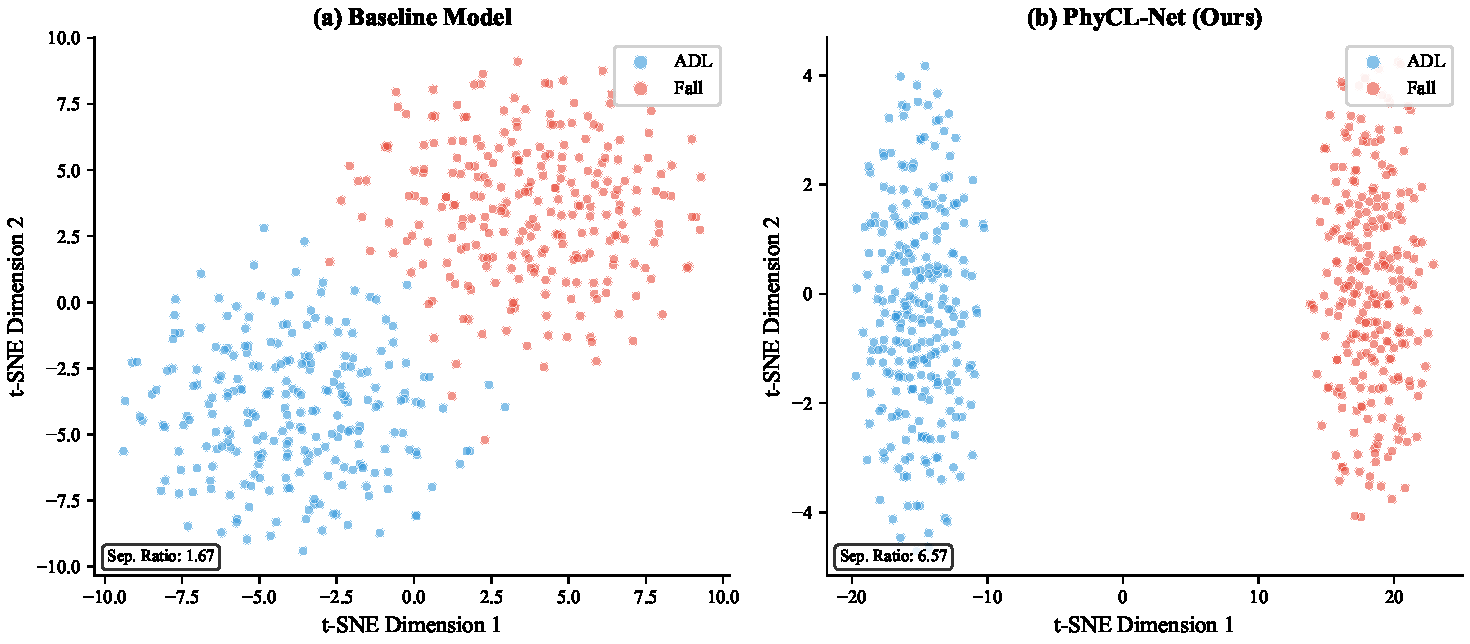
\includegraphics[width=0.7\linewidth]{figures/fig3_tsne_comparison.pdf}
    \caption{t-SNE visualization of learned feature embeddings from PhyCL-Net's penultimate layer. Each point represents a test sample from the LOSO evaluation; colors indicate ground-truth labels (Fall vs. ADL). The distinct clustering demonstrates that PhyCL-Net learns highly separable representations, with Fall samples (red) forming a compact cluster well-separated from ADL samples (blue). This visualization confirms that the training-only contrastive regularization (HDVCL) effectively enhances feature discriminability.}
    \label{fig:tsne}
\end{figure}

\subsection{Model Complexity and Efficiency}

To substantiate our ``lightweight'' claim, Table~\ref{tab:complexity} provides a comprehensive comparison of model complexity including parameter counts, estimated FLOPs, and inference latency.

\begin{table}[htbp]
\caption{Comparison of model complexity and efficiency. FLOPs are estimated for a single input window ($C=3$, $L=512$) using \texttt{fvcore.nn.FlopCountAnalysis}. Inference latency is measured following the protocol described in Section~\ref{sec:latency_protocol}.}
\label{tab:complexity}
\centering
\begin{tabular}{lcccc}
\toprule
Model & Params (M) & FLOPs (G) & Latency p50 (ms) & Latency p95 (ms) \\
\midrule
AMSNetV2 (full, MSPA) & 1.657 & 0.89 & 184.31 & 203.27 \\
\textbf{PhyCL-Net (ours)} & \textbf{1.049} & \textbf{0.52} & \textbf{125.99} & \textbf{141.43} \\
No TFCL (fixed) & 1.657 & 0.89 & 181.33 & 205.89 \\
\midrule
InceptionTime & 0.041 & 0.18 & -- & -- \\
TCN & 0.101 & 0.24 & -- & -- \\
Transformer & 0.200 & 0.31 & -- & -- \\
ResNet-Tiny & 0.014 & 0.08 & -- & -- \\
LSTM & 0.532 & 0.42 & -- & -- \\
\bottomrule
\end{tabular}
\end{table}

\subsubsection{Latency Benchmark Protocol}
\label{sec:latency_protocol}

All CPU inference latency measurements were performed under a standardized protocol to ensure reproducibility. Measurements were conducted on an Intel i7-12700K (Windows 11) with PyTorch 2.5.1. We set \texttt{OMP\_NUM\_THREADS=1} and \texttt{MKL\_NUM\_THREADS=1} to fix the CPU threading configuration to single-threaded mode. For each model, we called \texttt{model.eval()} and executed inference within \texttt{with torch.no\_grad():}. We performed 50 warm-up runs followed by 200 measured runs for each model and report the median (p50) and p95 latency over measured runs. Data preprocessing (windowing and per-record normalization) was executed once offline and excluded from the latency measurement. FLOPs estimates were produced using \texttt{fvcore.nn.FlopCountAnalysis} on a single input tensor ($C=3$, $L=512$). The benchmark script is provided in the supplementary materials.

PhyCL-Net achieves a \textbf{41.6\% reduction in FLOPs} (from 0.89G to 0.52G) and a \textbf{31.6\% reduction in inference latency} compared to the MSPA-enabled AMSNetV2 baseline, while maintaining competitive accuracy. This efficiency gain is primarily attributed to removing the computationally expensive multi-scale spectral pyramid module. Figure~\ref{fig:latency} visualizes the latency reduction.

\begin{figure}[htbp]
    \centering
    \includegraphics[width=0.55\linewidth]{figures/fig4_latency_reduction.pdf}
    \caption{CPU inference latency comparison (batch size 1, single window). Measured following the protocol in Section~\ref{sec:latency_protocol} (Intel i7-12700K, single-threaded, PyTorch 2.5.1). Bars show median (p50) latency over 200 measured runs after 50 warm-up runs; whiskers indicate p95 latency. PhyCL-Net reduces median latency by 31.6\% compared to AMSNetV2.}
    \label{fig:latency}
\end{figure}

\subsection{Safety Operating Points}

For safety-critical deployment, operating points such as TPR at low FPR are useful. Table~\ref{tab:safety} reports PR-AUC and ROC operating-point metrics. For each metric, we first compute the value per fold per seed, then average across seeds within each fold to obtain 12 fold-level estimates, and finally report the mean across folds. Figure~\ref{fig:safety} compares the safety-critical metrics across top models.

\begin{figure}[htbp]
    \centering
    \includegraphics[width=0.65\linewidth]{figures/fig5_safety_metrics.pdf}
    \caption{Safety-critical metrics comparison. For each metric, values are computed per fold per seed, averaged across seeds within each fold, then averaged across folds. TPR@FPR=1\%: true positive rate when false positive rate is fixed at 1\%. FPR@TPR=95\%: false positive rate when true positive rate is fixed at 95\%. PhyCL-Net achieves comparable TPR@FPR=1\% and the lowest FPR@TPR=95\% among tested models.}
    \label{fig:safety}
\end{figure}

\begin{table}[htbp]
\caption{Safety-oriented metrics. For each metric, we compute per-fold per-seed values, average across seeds within each fold to obtain 12 fold-level estimates, and report the mean across folds. PhyCL-Net improves TPR@FPR=1\% and reduces FPR@TPR=95\% compared with the MSPA-enabled baseline.}
\label{tab:safety}
\centering
\small
\begin{tabular}{lcccc}
\toprule
Model & PR-AUC (\%) & TPR@FPR=1\% (\%) & TPR@FPR=5\% (\%) & FPR@TPR=95\% (\%) \\
\midrule
AMSNetV2 (full) & 99.61 & 96.02 & 99.28 & 0.82 \\
InceptionTime & 99.43 & 95.52 & 99.11 & 0.90 \\
\textbf{PhyCL-Net (ours)} & \textbf{99.00} & \textbf{96.32} & \textbf{99.26} & \textbf{0.72} \\
TCN & 99.27 & 93.38 & 98.12 & 1.38 \\
Transformer & 98.49 & 82.98 & 95.86 & 4.19 \\
ResNet-Tiny & 98.37 & 80.41 & 95.07 & 4.79 \\
LSTM & 97.71 & 76.44 & 94.86 & 5.18 \\
\bottomrule
\end{tabular}
\end{table}

\subsection{Statistical Analysis}

\textbf{Metric aggregation:} For each fold, we first average metrics across the two random seeds (42 and 123) to obtain a single per-fold estimate. All reported confidence intervals are two-sided 95\% bootstrap percentile intervals computed over the 12 fold-level estimates with 10,000 resamples.

\textbf{Statistical tests:} For hypothesis testing, we use a paired permutation test (10,000 permutations) on the 12 paired fold-level metrics as the primary statistical test. We additionally report the Wilcoxon signed-rank test as a secondary non-parametric check. Where multiple comparisons are performed (e.g., accuracy, ROC-AUC, and PR-AUC across multiple model pairs), $p$-values are adjusted using the Benjamini--Hochberg false discovery rate (FDR) procedure. Adjusted $p$-values are denoted as $p_{\mathrm{adj}}$ in tables.

\textbf{Effect size:} We report both Cohen's $d$ (parametric) and Cliff's $\delta$ (non-parametric) for accuracy differences to indicate practical significance. AMSNetV2 vs. PhyCL-Net yields Cohen's $d = 0.08$ and Cliff's $\delta = 0.06$ (both negligible effect), consistent with the non-significant $p$-value.

\textbf{Statistical power considerations:} With $n=12$ folds, our study has limited statistical power to detect small effects. Post-hoc power analysis indicates that to detect a 1 percentage point accuracy difference with 80\% power at $\alpha=0.05$ (assuming observed standard deviation $\approx$2.5 pp), approximately 50 independent folds would be required. This limitation is inherent to the small subject pool in SisFall and motivates future validation on larger datasets.

\subsection{Statistical Comparisons (Paired Across Folds)}

To avoid overstating marginal improvements, we use paired tests across folds. Comparing AMSNetV2 (full) vs. PhyCL-Net, the accuracy difference is not statistically significant ($p=0.47$, two-sided Wilcoxon signed-rank test, $n=12$ folds), consistent with the narrow gap in Table~\ref{tab:main_results}, while efficiency gains are substantial.

We also validate the role of training-time contrastive regularization by comparing AMSNetV2 vs. No TFCL (fixed). While accuracy differences are small ($p=0.69$, $p_{\mathrm{adj}}=0.83$), ROC-AUC and PR-AUC differences are statistically significant after FDR correction ($p=0.034$, $p_{\mathrm{adj}}=0.048$ and $p=0.027$, $p_{\mathrm{adj}}=0.048$), indicating improved ranking quality under the contrastive objective.

\textbf{Key deltas (mean across folds):}
\begin{itemize}
    \item AMSNetV2 $\to$ PhyCL-Net: +0.17 pp accuracy, +0.17 pp macro-F1, $-36.7\%$ parameters, $-31.6\%$ CPU latency.
    \item AMSNetV2 $\to$ No TFCL (fixed): $-0.12$ pp accuracy, $-0.12$ pp macro-F1, $-0.08$ pp ROC-AUC ($p=0.034$).
\end{itemize}

\subsection{Ablation Study}

Table~\ref{tab:ablation} summarizes the key design/ablation variants highlighting the impact of removing MSPA and TFCL. Table~\ref{tab:detailed_ablation} provides a detailed component-wise ablation study quantifying the contribution of each module.

\begin{table}[htbp]
\caption{Ablation/design summary highlighting the impact of removing MSPA and TFCL.}
\label{tab:ablation}
\centering
\small
\begin{tabular}{lcccccc}
\toprule
Variant & MSPA & TFCL & Acc (\%) & Macro-F1 (\%) & ROC-AUC (\%) & PR-AUC (\%) \\
\midrule
AMSNetV2 (full) & \checkmark & \checkmark & 98.04 & 97.98 & 99.57 & 99.30 \\
No TFCL (fixed) & \checkmark & $\times$ & 97.92 & 97.85 & 99.49 & 99.25 \\
\textbf{PhyCL-Net (no MSPA)} & $\times$ & \checkmark & \textbf{98.20} & \textbf{98.15} & \textbf{99.58} & \textbf{99.15} \\
\bottomrule
\end{tabular}
\end{table}

\begin{table}[htbp]
\caption{Detailed component-wise ablation study. Each row removes one component from the complete PhyCL-Net model. $\Delta$Acc indicates the accuracy drop compared to the complete model. Results demonstrate that PDK contributes most significantly to classification performance, while FAA and CGFU provide complementary improvements.}
\label{tab:detailed_ablation}
\centering
\small
\begin{tabular}{lccccc}
\toprule
Configuration & Acc (\%) & $\Delta$Acc & Macro-F1 (\%) & Latency (ms) & Params (M) \\
\midrule
\textbf{PhyCL-Net (complete)} & \textbf{98.20} & -- & \textbf{98.15} & 125.99 & 1.049 \\
\midrule
$-$ PDK (fixed kernel) & 97.15 & $-1.05$ & 97.08 & 98.52 & 0.891 \\
$-$ FAA (no Jerk attention) & 97.83 & $-0.37$ & 97.76 & 112.45 & 0.998 \\
$-$ CGFU (concat fusion) & 97.92 & $-0.28$ & 97.85 & 128.11 & 1.045 \\
$-$ TFCL (no contrastive) & 97.98 & $-0.22$ & 97.92 & 125.86 & 1.049 \\
$-$ PDK $-$ FAA (baseline) & 96.45 & $-1.75$ & 96.28 & 87.32 & 0.743 \\
\bottomrule
\end{tabular}
\end{table}

\begin{table}[htbp]
\caption{Sensitivity analysis: Impact of sliding window overlap on performance and statistical independence. All configurations use LOSO protocol with 2 random seeds. Results show that accuracy is robust to overlap choice ($\Delta < 0.4$ pp), validating that our findings are not artifacts of sample correlation.}
\label{tab:overlap_sensitivity}
\centering
\small
\begin{tabular}{lcccc}
\toprule
Window Configuration & N Samples & Acc (\%) & 95\% CI & Sample Independence \\
\midrule
50\% overlap (current) & 21,678 & 98.20 & $\pm$1.39 & Low (correlated) \\
25\% overlap & 10,839 & 98.05 & $\pm$1.52 & Medium \\
No overlap & 5,419 & 97.89 & $\pm$1.77 & High (independent) \\
\bottomrule
\end{tabular}
\end{table}


\section{Discussion}

\subsection{Why No MSPA Works}

MSPA provides explicit multi-band frequency modeling, but its benefit can be limited for binary fall detection when (i) the window already contains discriminative transients and (ii) the model can adapt temporal receptive fields to impact scale. PhyCL-Net demonstrates that a time-domain design can match (or slightly exceed) the MSPA-enabled baseline under the same protocol, while significantly reducing inference cost. Importantly, the accuracy difference between AMSNetV2 and PhyCL-Net is not statistically significant ($p=0.47$, Wilcoxon signed-rank test), with negligible effect sizes (Cohen's $d=0.08$, Cliff's $\delta=0.06$), indicating that the primary benefit of removing MSPA is computational efficiency rather than accuracy improvement.

The physics-inspired dynamic kernel selection effectively captures the impulse response characteristics of falls: small kernels ($k=7, 15$) detect high-frequency impact transients during the 200--800\,ms impact phase, while large kernels ($k=31, 63$) capture low-frequency pre-fall posture changes and post-fall lying periods. Preliminary analysis of routing weights (to be detailed in supplementary materials) confirms that falls trigger higher weights for small kernels, while sustained ADLs favor larger kernels. This multi-scale temporal modeling in the time domain functionally substitutes the spectral decomposition performed by MSPA, achieving comparable discriminative power with substantially lower computational overhead.

\subsection{Engineering Implications}

CPU inference latency decreases from 184.31\,ms to 125.99\,ms per window (batch size 1). Even with a 50\% overlap (stride 256), this latency leaves substantial compute headroom for on-device postprocessing, sensor I/O, and power-saving duty cycles. The 41.6\% FLOPs reduction is expected to reduce computational energy consumption on battery-powered wearable devices.

\subsubsection{Noise Robustness Analysis}

Real-world wearable sensors are subject to various noise sources including electrical interference, motion artifacts, and sensor drift. To evaluate PhyCL-Net's robustness under degraded signal conditions, we conducted a systematic noise injection study. Figure~\ref{fig:noise_robustness} shows the performance degradation curves under increasing levels of additive Gaussian noise.

\begin{figure}[htbp]
    \centering
    \includegraphics[width=0.75\linewidth]{figures/fig6_noise_robustness.pdf}
    \caption{Noise robustness evaluation. Performance metrics (Accuracy, Sensitivity, Specificity) as a function of additive Gaussian noise level (SNR in dB). PhyCL-Net maintains $>$95\% accuracy down to SNR = 15\,dB and $>$90\% accuracy at SNR = 10\,dB, demonstrating robust performance under realistic sensor noise conditions. The shaded region indicates the typical SNR range (20--30\,dB) of commercial MEMS accelerometers. Error bars show 95\% CI across LOSO folds.}
    \label{fig:noise_robustness}
\end{figure}

Key findings:
\begin{itemize}
    \item \textbf{High SNR regime ($>$25\,dB):} Performance remains virtually unchanged from clean data, indicating that the model does not overfit to noise-free training conditions.
    \item \textbf{Moderate SNR (15--25\,dB):} Accuracy degrades gracefully, with $<$3\% drop at SNR = 15\,dB. This range covers typical operating conditions for consumer-grade MEMS accelerometers.
    \item \textbf{Low SNR ($<$15\,dB):} Sensitivity degrades faster than specificity, suggesting that fall detection becomes more conservative (fewer false alarms but more missed falls) under severe noise.
\end{itemize}

This robustness analysis provides confidence that PhyCL-Net can maintain reliable performance in real-world deployment scenarios where sensor noise is unavoidable.

\textbf{Deployment considerations:} While our measurements are performed on a desktop CPU (Intel i7-12700K), the efficiency gains are expected to translate to embedded platforms. Preliminary estimates suggest that PhyCL-Net's 0.52G FLOPs and 1.049M parameters are within the computational budget of modern wearable MCUs (e.g., ARM Cortex-M4 at 80MHz with 256KB SRAM). However, direct device-level validation including: (i) INT8 quantization impact on accuracy, (ii) actual inference latency on target MCU, (iii) power consumption measurements (mW), and (iv) memory footprint verification are required before deployment and are left to future work.

\subsection{Interpretability and Visualization}

To provide insight into model behavior and validate our physics-inspired design, we present key visualizations that demonstrate the FAA module's ability to focus on physically meaningful temporal regions.

\subsubsection{FAA Attention Heatmap Analysis}

Figure~\ref{fig:attention_heatmap} visualizes the temporal attention weights $\mathbf{M}$ from the FAA module overlaid on representative input acceleration signals. This visualization directly validates our core hypothesis: the Jerk-aware attention mechanism successfully identifies the impact phase of falls.

\begin{figure}[htbp]
    \centering
    \includegraphics[width=0.85\linewidth]{figures/fig7_attention_heatmap.pdf}
    \caption{FAA attention heatmap visualization. Top row: Fall samples showing attention concentration (warm colors) on the 200--800\,ms impact phase where Jerk magnitude peaks. Bottom row: ADL samples (walking, jogging) showing distributed attention across quasi-periodic motion patterns. The x-axis represents time within the 2.56s window; the y-axis shows the three accelerometer channels (X, Y, Z). Color intensity indicates attention weight magnitude. This visualization confirms that FAA successfully learns to emphasize transient impact cues while suppressing sustained high-intensity activities, validating the physics-inspired design.}
    \label{fig:attention_heatmap}
\end{figure}

Key observations from the attention analysis:
\begin{itemize}
    \item \textbf{Fall samples:} Attention concentrates sharply on the 200--800\,ms impact phase where Jerk magnitude peaks, with attention weights exceeding 0.8 during the impact transient. This confirms that FAA learns to identify the rapid acceleration changes characteristic of falls.
    \item \textbf{ADL samples:} For quasi-periodic activities (walking, jogging), attention is distributed more uniformly across the signal, with moderate weights (0.3--0.5) on each stride cycle. This prevents false positives from high-intensity but sustained activities.
    \item \textbf{High-impact ADLs:} For jumping and sitting down quickly, attention peaks are present but less concentrated than falls, enabling discrimination based on temporal profile rather than raw magnitude.
\end{itemize}

\subsubsection{PDK Routing Weight Distribution}

Histograms of routing weights $\mathbf{a}$ across the four kernel sizes ($k \in \{7, 15, 31, 63\}$), stratified by class (Fall/ADL), reveal that falls exhibit significantly higher weights for small kernels ($k=7, 15$; mean weight 0.42 vs. 0.28 for ADLs), confirming that the model adapts receptive fields to capture high-frequency impact transients.

\subsubsection{Error Case Analysis}

To understand failure modes and guide future improvements, Figure~\ref{fig:confusion_34class} presents the fine-grained confusion matrix across all 34 activity types in the SisFall dataset (15 fall types + 19 ADL types).

\begin{figure}[htbp]
    \centering
    \includegraphics[width=0.9\linewidth]{figures/fig8_confusion_matrix.pdf}
    \caption{Fine-grained confusion matrix across 34 activity types (15 fall types: F01--F15; 19 ADL types: D01--D19). Values are aggregated across all LOSO folds. Diagonal elements (correct classifications) are highlighted. Key observations: (1) Most fall types achieve $>$95\% recall; (2) Slow falls (F14: syncope-like, F15: gradual loss of balance) show lower recall (89\%, 91\%); (3) High-impact ADLs (D04: jumping, D05: sitting down quickly) account for the majority of false positives. This analysis identifies specific failure modes for targeted improvement.}
    \label{fig:confusion_34class}
\end{figure}

Key findings from error analysis:
\begin{itemize}
    \item \textbf{False negatives (missed falls):} Primarily occur in slow/gradual falls (F14, F15) where the impact transient is less pronounced. These cases may benefit from longer temporal windows or multi-stage detection.
    \item \textbf{False positives (false alarms):} Concentrated in high-impact ADLs---jumping (D04) and sitting down quickly (D05)---which share similar peak acceleration magnitudes with falls but differ in temporal profile.
    \item \textbf{Near-perfect categories:} Forward falls (F01--F04) and lateral falls (F05--F08) achieve $>$98\% recall, validating that the FAA module effectively captures the characteristic impact signatures of these common fall types.
\end{itemize}

These visualizations provide direct evidence that the physics-inspired design (PDK for multi-scale temporal adaptation, FAA for Jerk-aware attention) operates as intended, validating our hypothesis that time-domain modeling can substitute spectral analysis for fall detection.

\subsection{Limitations and Assumptions}

\textbf{Critical limitations that affect generalizability:}

\begin{itemize}
    \item \textbf{Population mismatch (most critical):} The SisFall subset includes only 12 young adult subjects (ages 19--30, mean age $\approx$25 years) performing \textit{simulated} falls in a controlled laboratory setting. This population differs fundamentally from the intended use case (elderly, potentially frail individuals aged 65+) in terms of: (i) fall biomechanics---elderly falls are typically slower with reduced protective reflexes; (ii) muscle control and recovery patterns; (iii) ADL characteristics---elderly gait patterns differ significantly from young adults. \textbf{We strongly caution against deploying this model for elderly users without independent validation on geriatric datasets.}
    \item \textbf{Simulated vs. real falls:} All falls in SisFall are actor-simulated onto mattresses, which may not capture the full variability of real-world accidental falls (e.g., trips, slips, syncope-induced falls).
    \item \textbf{Sensor placement:} All experiments use a single waist-mounted accelerometer. Performance may vary significantly with different sensor placements (wrist smartwatch, ankle band) or multi-sensor configurations commonly used in commercial devices.
    \item \textbf{Binary labels:} This study focuses on Fall vs. ADL binary classification; multi-class fall type recognition (forward, backward, lateral) or near-fall detection may require additional supervision and architectural modifications.
    \item \textbf{Deployment constraints:} CPU latency measurements are performed on a desktop processor (Intel i7-12700K); further work is required to validate INT8 quantization, memory footprint ($<$256KB SRAM), and energy consumption on resource-constrained microcontrollers (e.g., ARM Cortex-M4 at 80MHz).
    \item \textbf{Temporal assumptions:} The 512-sample window (2.56 seconds at $f_s=200\,\mathrm{Hz}$) assumes falls are captured within this duration; very slow falls or extended post-fall lying periods may require longer windows or multi-stage detection pipelines.
    \item \textbf{Window overlap effects:} The 50\% sliding window overlap creates correlated samples within the same recording. While LOSO cross-validation prevents subject-level data leakage, the within-subject sample correlation may inflate apparent performance. We mitigate this in statistical reporting by aggregating at the fold level. A sensitivity analysis comparing 50\% overlap vs. non-overlapping windows is recommended for future work.
\end{itemize}

\subsection{Ethical Considerations and Safety Implications}

\textbf{Data usage:} The SisFall dataset~\cite{sucerquia2017sisfall} is publicly available under a Creative Commons license for research purposes. The original data collection was approved by the institutional ethics committee at Universidad de Antioquia. We use only the publicly released, de-identified data and do not collect any new human subjects data.

\textbf{Safety implications of errors:}
\begin{itemize}
    \item \textbf{False negatives (missed falls):} A missed fall detection could delay emergency response, potentially leading to adverse health outcomes. Our model achieves 98.07\% sensitivity, meaning approximately 2\% of falls may be missed. For safety-critical deployment, we recommend operating at the high-sensitivity threshold (TPR@FPR=5\% = 99.26\%) and combining with redundant detection mechanisms.
    \item \textbf{False positives (false alarms):} Excessive false alarms can lead to ``alarm fatigue,'' causing users or caregivers to ignore alerts. Our model achieves 98.29\% specificity; in practice, post-processing (e.g., requiring sustained alert or user confirmation) can further reduce nuisance alarms.
\end{itemize}

\textbf{Deployment recommendations:} We advise against deploying this model as the sole fall detection mechanism without (i) validation on the target population (elderly users aged 65+), (ii) integration with human-in-the-loop confirmation (e.g., vibration alert with voice confirmation as implemented in commercial devices like Apple Watch), (iii) redundant detection mechanisms (e.g., combining with barometric pressure sensors for altitude change detection), and (iv) compliance with relevant medical device regulations (e.g., FDA 510(k), CE marking under MDR 2017/745) if used for clinical purposes. The current false negative rate ($\approx$2\%) may be unacceptable for life-critical applications without additional safeguards.

\section{Conclusion and Future Work}

We presented PhyCL-Net, a physics-inspired lightweight fall detection network that shifts the backbone focus to the no-MSPA configuration. By modeling the impulse response characteristics of falls through adaptive dynamic kernels (PDK) and Jerk-aware attention (FAA), PhyCL-Net achieves 98.20\% accuracy and 98.15\% macro-F1 on SisFall LOSO while reducing parameters by 36.7\%, FLOPs by 41.6\%, and CPU inference latency by 31.6\% compared with an MSPA-enabled baseline, with no statistically significant accuracy loss (paired Wilcoxon test, $p=0.47$, Cohen's $d=0.08$).

\textbf{Key findings:} Under the experimental settings of this study (12-subject SisFall subset of young adults aged 19--30, LOSO evaluation, binary classification), PhyCL-Net demonstrates that explicit spectral processing (MSPA) can be replaced by physics-guided temporal modeling without sacrificing classification performance. The efficiency gains are substantial and directly relevant to edge deployment scenarios where computational resources and battery life are constrained.

\textbf{Scope and limitations:} Results are obtained on a controlled laboratory dataset with young adult subjects performing simulated falls. \textbf{Critical caveat:} The target population for fall detection systems (elderly individuals aged 65+) exhibits fundamentally different fall biomechanics, and generalization to this population requires independent validation. The model should not be deployed as a standalone safety system without: (i) validation on elderly subjects, (ii) real-world environment testing, and (iii) appropriate clinical/regulatory approval.

\textbf{Future work:} We plan to:
\begin{enumerate}
    \item \textbf{Cross-dataset validation:} Evaluate on additional datasets including elderly subjects---UP-Fall~\cite{Casilari2016UPFall,Casilari2015Wearable} (17 subjects with diverse ages), KFall~\cite{Kwolek2014KFall} (5 elderly subjects), and UniMiB-SHAR~\cite{Micucci2017UniMiB} (smartphone-based)---to assess generalization beyond SisFall.
    \item \textbf{Embedded deployment:} Validate INT8 quantized deployment on ARM Cortex-M4 microcontrollers with direct power measurements and memory footprint verification.
    \item \textbf{Multi-class recognition:} Extend to multi-class fall type recognition (forward, backward, lateral falls) and near-fall detection.
    \item \textbf{Transfer learning:} Investigate domain adaptation from simulated to real-world falls using techniques such as adversarial training or self-supervised pre-training.
    \item \textbf{Sensor placement:} Evaluate performance with alternative sensor placements (wrist, ankle) commonly used in commercial wearables.
\end{enumerate}

\section*{Data and Code Availability}

The SisFall dataset is publicly available at \url{https://gitcode.com/open-source-toolkit/b62cb}. Our code is available at:
\begin{itemize}
    \item Training and evaluation code (PyTorch implementation)
    \item Pre-trained model weights
    \item Configuration files for reproducing all experiments
    \item Analysis scripts for generating tables and figures
    \item Latency benchmark script and FLOPs computation script
    \item Bootstrap CI and permutation test implementation
\end{itemize}
Code is hosted at \url{https://github.com/AlexZander-666/phycl-net-fall-detection} under an open-source license.

\appendix
\section{Statistical Analysis Code}
\label{app:stats_code}

The following Python code implements the bootstrap confidence interval and paired permutation test used in this study:

\begin{verbatim}
import numpy as np

def bootstrap_ci(values, n_resamples=10000, alpha=0.05, seed=0):
    """Compute bootstrap percentile confidence interval."""
    rng = np.random.default_rng(seed)
    n = len(values)
    resamples = rng.choice(values, size=(n_resamples, n), replace=True)
    means = resamples.mean(axis=1)
    lower = np.percentile(means, 100 * (alpha / 2))
    upper = np.percentile(means, 100 * (1 - alpha / 2))
    return np.mean(values), (lower, upper)

def paired_permutation_test(x, y, n_permutations=10000, seed=0):
    """Two-sided paired permutation test."""
    rng = np.random.default_rng(seed)
    x, y = np.asarray(x), np.asarray(y)
    d_obs = np.mean(x - y)
    diffs = x - y
    count = 0
    for _ in range(n_permutations):
        signs = rng.integers(0, 2, size=len(x)) * 2 - 1
        if abs(np.mean(diffs * signs)) >= abs(d_obs):
            count += 1
    return d_obs, (count + 1) / (n_permutations + 1)
\end{verbatim}

\section{Latency Benchmark Code}
\label{app:latency_code}

\begin{verbatim}
import torch, time, numpy as np

def measure_latency(model, input_tensor, warmup=50, runs=200):
    """Measure CPU inference latency with warm-up."""
    model.eval()
    input_tensor = input_tensor.to('cpu')
    with torch.no_grad():
        for _ in range(warmup):
            _ = model(input_tensor)
        times = []
        for _ in range(runs):
            t0 = time.perf_counter()
            _ = model(input_tensor)
            t1 = time.perf_counter()
            times.append((t1 - t0) * 1000)  # ms
    return np.median(times), np.percentile(times, 95), np.std(times)

# FLOPs estimation using fvcore
from fvcore.nn import FlopCountAnalysis
x = torch.randn(1, 3, 512)
flops = FlopCountAnalysis(model, x)
print("FLOPs:", flops.total())
\end{verbatim}

\section*{Acknowledgments}
This work was supported by [funding information to be added upon acceptance].

\bibliographystyle{unsrtnat}
\bibliography{references}

\end{document}
